% Titre de la partie
\section[Pratique]{Application sur la Crimes Database Chicago Police Department}

%%%%%%%%%%%%%%%%%%%%%%%%%%%%%%%%%%%%%%%%%%%%%%%%
% Première diapo (avec des équations)
%%%%%%%%%%%%%%%%%%%%%%%%%%%%%%%%%%%%%%%%%%%%%%%%
\begin{frame}
	\frametitle{Présentation de la base de données}
	\framesubtitle{Chicago Crimes Database 2020}
		\begin{figure}
			    \centering
				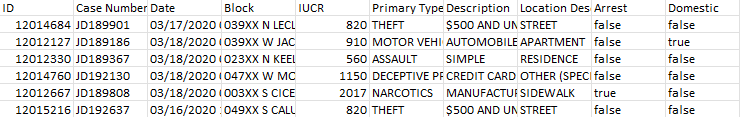
\includegraphics[width=1.0\linewidth]{figures/database.png}
			
		\end{figure}
            \begin{figure}
			    \centering
				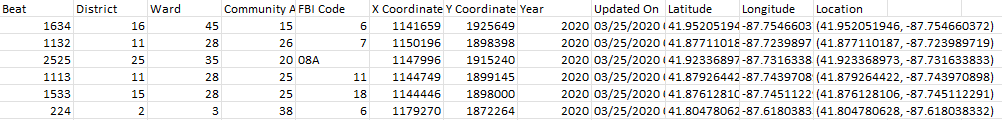
\includegraphics[width=1.0\linewidth]{figures/database2.png}
			
		\end{figure}
\end{frame}

\begin{frame}
	\frametitle{Présentation de la base de données}
	\framesubtitle{Filtrage de la base de données}
 \begin{block}{Filtrage}
    \begin{itemize}
            \item Supprimer les lignes avec des données manquantes
            \item Conserver uniquement les cambriolages
            \item Conserver uniquement les colonnes suivantes : Date, Primary Type, Latitude et Longitude
        \end{itemize}

    \end{block}
\end{frame}

\begin{frame}
	\frametitle{Présentation de la base de données}
	\framesubtitle{Formatage de la base de données}
 \begin{block}{Formatage}
    \begin{itemize}
            \item Passage du format date US au format EU
            \item Trier les cambriolages par ordre chronologique
            \item Définition de l'instant $t_0$=0 correspondant à l'instant du 01/01/2020 à 00H00
        \end{itemize}

    \end{block}
\end{frame}

\begin{frame}
	\frametitle{Présentation de la base de données}
	\framesubtitle{Première analyse}
\begin{alertblock}{Problèmes rencontrés}
\begin{itemize}
            \item Liste trop longue 
            \item Valeurs des instants trop grandes
            \end{itemize}
	\end{alertblock}

 \begin{block}{Solutions exploitées}
 \begin{itemize}
            \item Restriction spatiale
            \item Changement échelle temporelle
            \end{itemize}
	\end{block}
\end{frame}

\begin{frame}
	\frametitle{Présentation de la base de données}
	\framesubtitle{Chicago Crimes Database 2020}
         \begin{block}{Affichage Chicago Map}
		\begin{figure}
			    \centering
				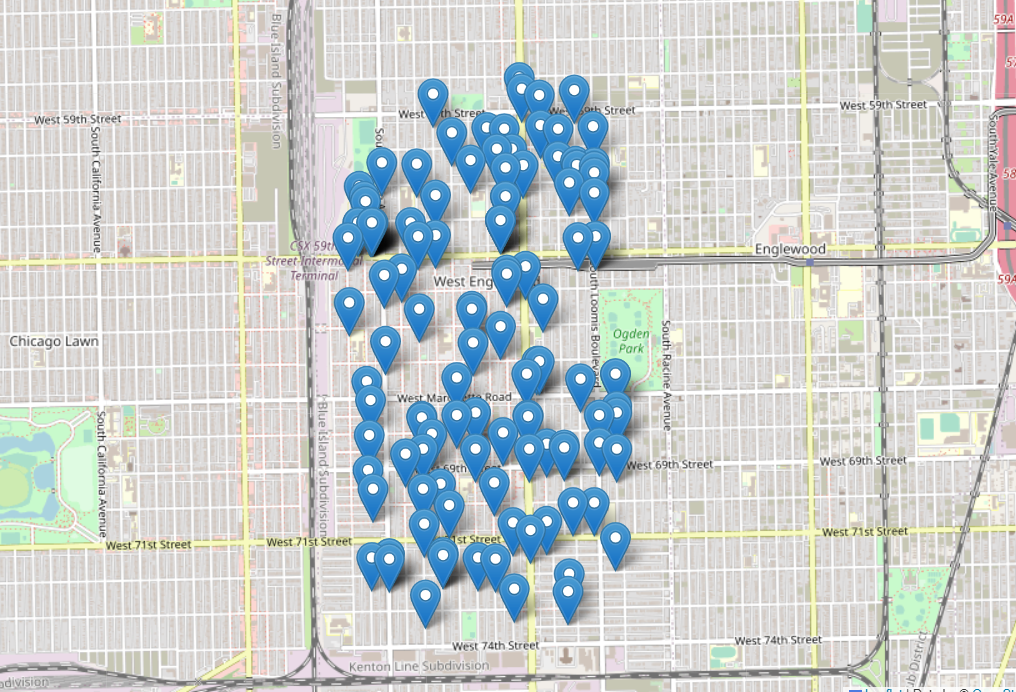
\includegraphics[width=0.8\linewidth]{figures/MAP.png}
			
		\end{figure}
  \end{block}
\end{frame}

\begin{frame}
	\frametitle{Présentation de la base de données}
	\framesubtitle{Premières estimations}
         \begin{block}{Estimations des paramètres}
         \begin{itemize}
            \item $\lambda_0$=0.3067893
            \item $\alpha$=0.11263505
            \item $\beta$=0.03089197
            \end{itemize}
  
  \end{block}

  \begin{block}{Estimations des cambriolages}
         \begin{itemize}
            \item Nombre réel: 125 
            \item Nombre simulé: 125
            \end{itemize}
  
  \end{block}
\end{frame}

\begin{frame}
    \frametitle{Application du modèle}
    \framesubtitle{}
        \begin{figure}
            \centering
            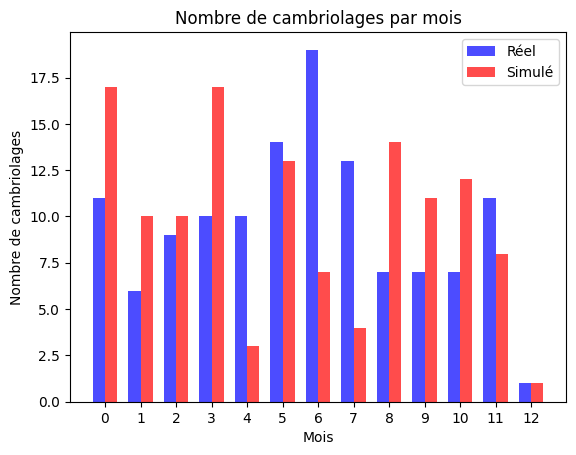
\includegraphics[width=0.6\linewidth]{figures/téléchargement (3).png}
        \end{figure}
\end{frame}

\begin{frame}
    \frametitle{Application du modèle}
    \framesubtitle{Exemple Fonction Calibrage(instants, 50)}
        \begin{figure}
            \centering
            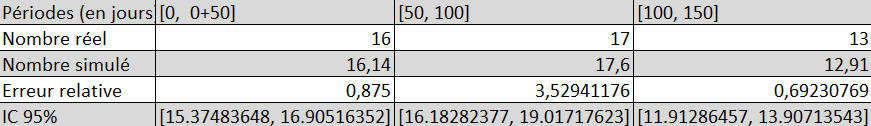
\includegraphics[width=1.0\linewidth]{figures/tab2.png}
        \end{figure}
        \begin{figure}
            \centering
            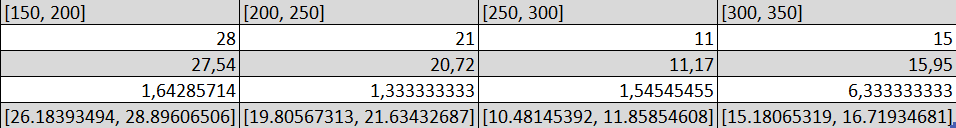
\includegraphics[width=1.0\linewidth]{figures/tab3.png}
        \end{figure}
\end{frame}

\begin{frame}
	\frametitle{Application du modèle}
	\framesubtitle{Calibrage}
         \begin{block}{Estimations des paramètres}
         \begin{itemize}
            \item $\lambda_0$=0.30990218
            \item $\alpha$=0.13504193
            \item $\beta$=0.02762651
            \end{itemize}
  
  \end{block}

    \begin{block}{Estimations des cambriolages}
         \begin{itemize}
            \item Nombre réel: 125 
            \item Nombre simulé: 123
            \end{itemize}
  
  \end{block}
\end{frame}

\begin{frame}
    \frametitle{Application du modèle}
    \framesubtitle{}
        \begin{figure}
            \centering
            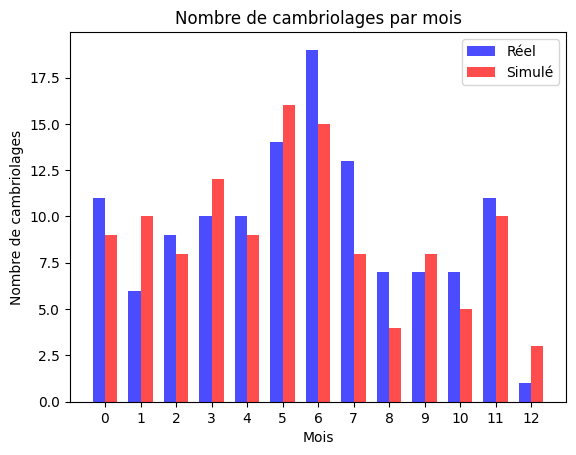
\includegraphics[width=0.6\linewidth]{figures/téléchargement (1).png}
        \end{figure}
\end{frame}

